\section{First iteration: desktop design}
\label{sec:iteration1}

The first iteration produced the desktop site that went live at osr.clarelab.moe on 11 June 2026 \cite{osr}.

\subsection{Design: personas and scenarios}

I designed for three personas and their scenarios \cite{benyon}. The primary one predates the product. The other two were sharpened after launch from the coded comment corpus but frame both iterations.

\textbf{P1, Chen Rui, 20, CS undergraduate planning a direct PhD abroad.} A second-year student at a mid-tier Chinese university, deciding which countries to shortlist before picking labs. He wants to compare countries on long-run settlement odds rather than admission odds, rank institutions by whether alumni stay, and justify the shortlist to his parents with numbers rather than forum anecdotes. His frustrations: evidence is anecdotal and scattered, composite rankings read as repackaged prestige lists, and definitions are under-explained (does a short trip home break \textbf{No return}?). He is desktop-first and will read a methodology page end to end.

His scenario. One evening he opens the mobility board, sets nationality to China, and is surprised that Australia shows the highest Stay when forums say that window closed after 2024. Before trusting the number he reads the right-censoring rule on the methodology page. He drills from country to city, then reads the R-tiers of his three candidate universities. One of them seems missing until he notices and disables the default flow-threshold filter. He screenshots two boards into his planning document and drops Japan for its low No return. Forty minutes replace a week of forum reading.

P1 is autobiographical (Section~\ref{sec:pact}), which explains the product's metric depth but biased the first iteration toward my own context: large screen, pointer, English, methodology-tolerant. The launch made that bias expensive. The secondary personas mark what P1 misses. \textbf{P2, Lin Xiaoyu, 24}, holds two taught-master's offers and needs to know how much researcher data transfers to her non-research case. She is phone-first, reached OSR inside the rednote app, and decides from boards and shared screenshots, not methodology text. Her scenario is first contact. She taps the launch post on her commute, lands on the mobility board on a six-inch screen inside the rednote WebView, sets nationality, pinches the map toward her two offer cities, reads each institution's tier next to its arrival mass, and screenshots the board into a group chat without ever seeing a desktop. Iteration 1 deferred that scenario. It became the spec and the test script of iteration 2 (Section~\ref{sec:iteration2}). \textbf{P3, Zhao Kai, 28}, a backend engineer planning an exit route, reads the board as a revealed-preference signal but decides on liveability, legal protections, and wages, which OSR does not carry. He keeps local copies of anything that might disappear. Full persona tables and scenarios are in Drive \texttt{06 Design library}.

\paragraph{Envisioning.} Before wireframing I explored a high-fidelity concept (Figure~\ref{fig:concept}), an analytics dashboard ranking institutions on a single composite score with an evidence badge and a detail pane. The dashboard-with-detail-pane skeleton survived into the shipped design. The composite score did not. I replaced it with three observable metrics (Arrival, Stay, No return) plus a Tier whose formula (recursive tertiles of the Stay/No-return mean) is itself inspectable. The launch vindicated this. Users challenged even directly observable percentages (14 metric-comprehension comments), and one dismissed the ranking as ``obviously just a university ranking''. A black-box score would have had no defence.

\begin{figure}[!t]
\centering
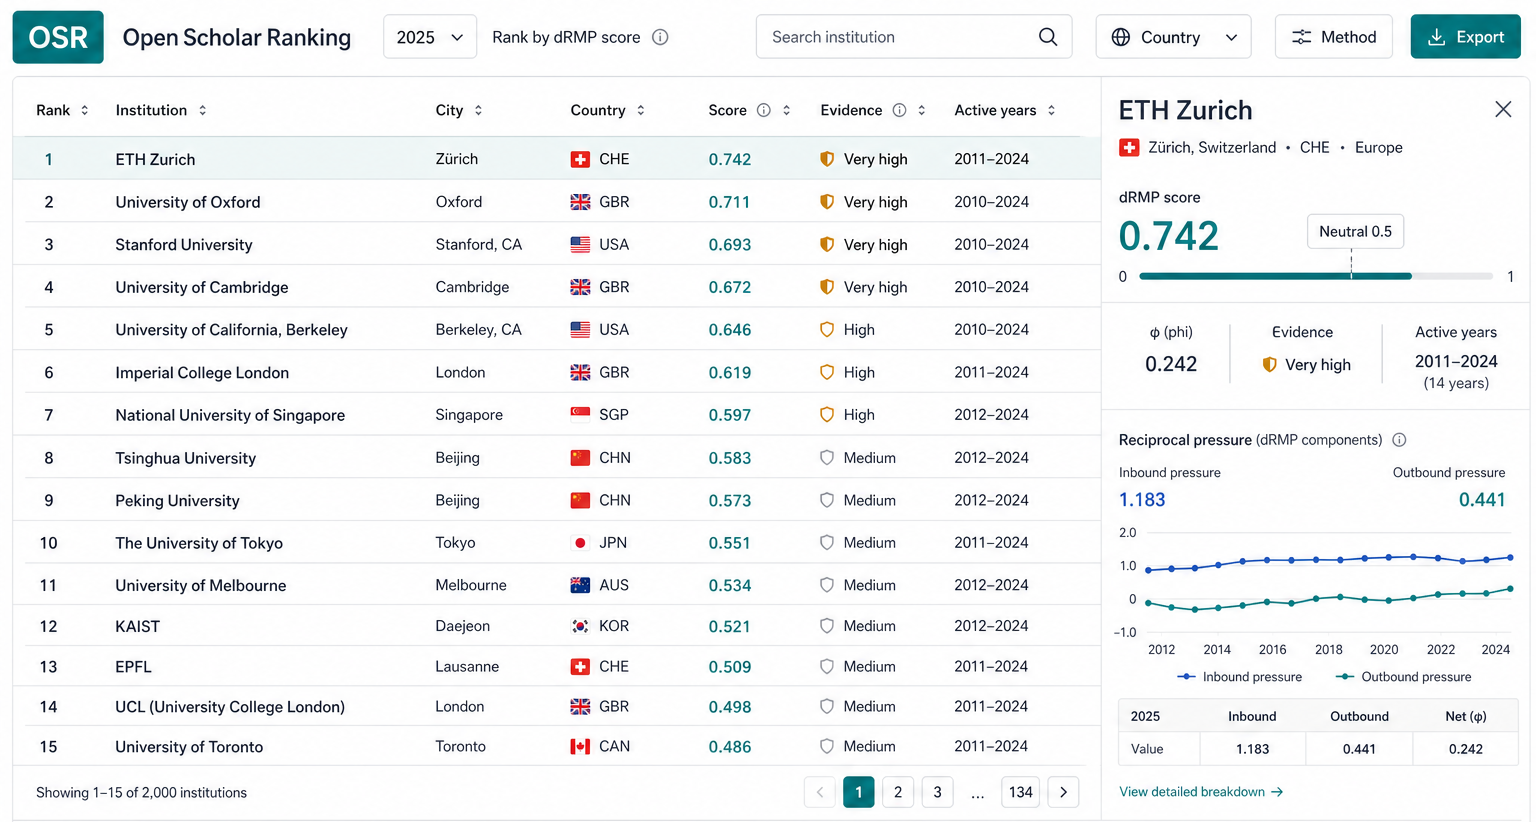
\includegraphics[width=0.72\linewidth]{figures/fig-concept-cropped.png}
\caption{Early high-fidelity concept, a dashboard ranking institutions on one composite score. The layout survived, but the opaque score was replaced by observable metrics.}
\label{fig:concept}
\end{figure}

\subsection{Prototyping}

Five low-fidelity wireframes, W1--W5, fixed the design's commitments before implementation (W1 shown here, W2--W5 in Drive \texttt{02 Prototype}). W1 (Figure~\ref{fig:w1}) is the mobility view. Map and destination board sit side by side under one shared filter state, where year, nationality, and geographic scope re-scope both panels at once, so a value on a map tag and in a board row can never disagree. A header checkbox picks which metric ranks the list. W2 swaps the right panel to institution rows and fixes the tier badges, an R1--R4 chip on every row, with chips and a search box filtering the table live. W3 carries this to the ranking page. Clicking a row opens a detail pane with rank, tier, and score trend, without a page change. W4 makes the third commitment concrete. Methodology sits one click from every metric. It glosses each metric in the same words the boards use, draws one scholar's trajectory to show what Arrival, Stay, and No return count, and renders censored years as hatched, never shown as zero. W5 sketches a phone layout (single column, no document scroll, columns drop before rows). The desktop-first implementation deferred it. The launch punished that deferral within hours.

\begin{figure}[!t]
\centering
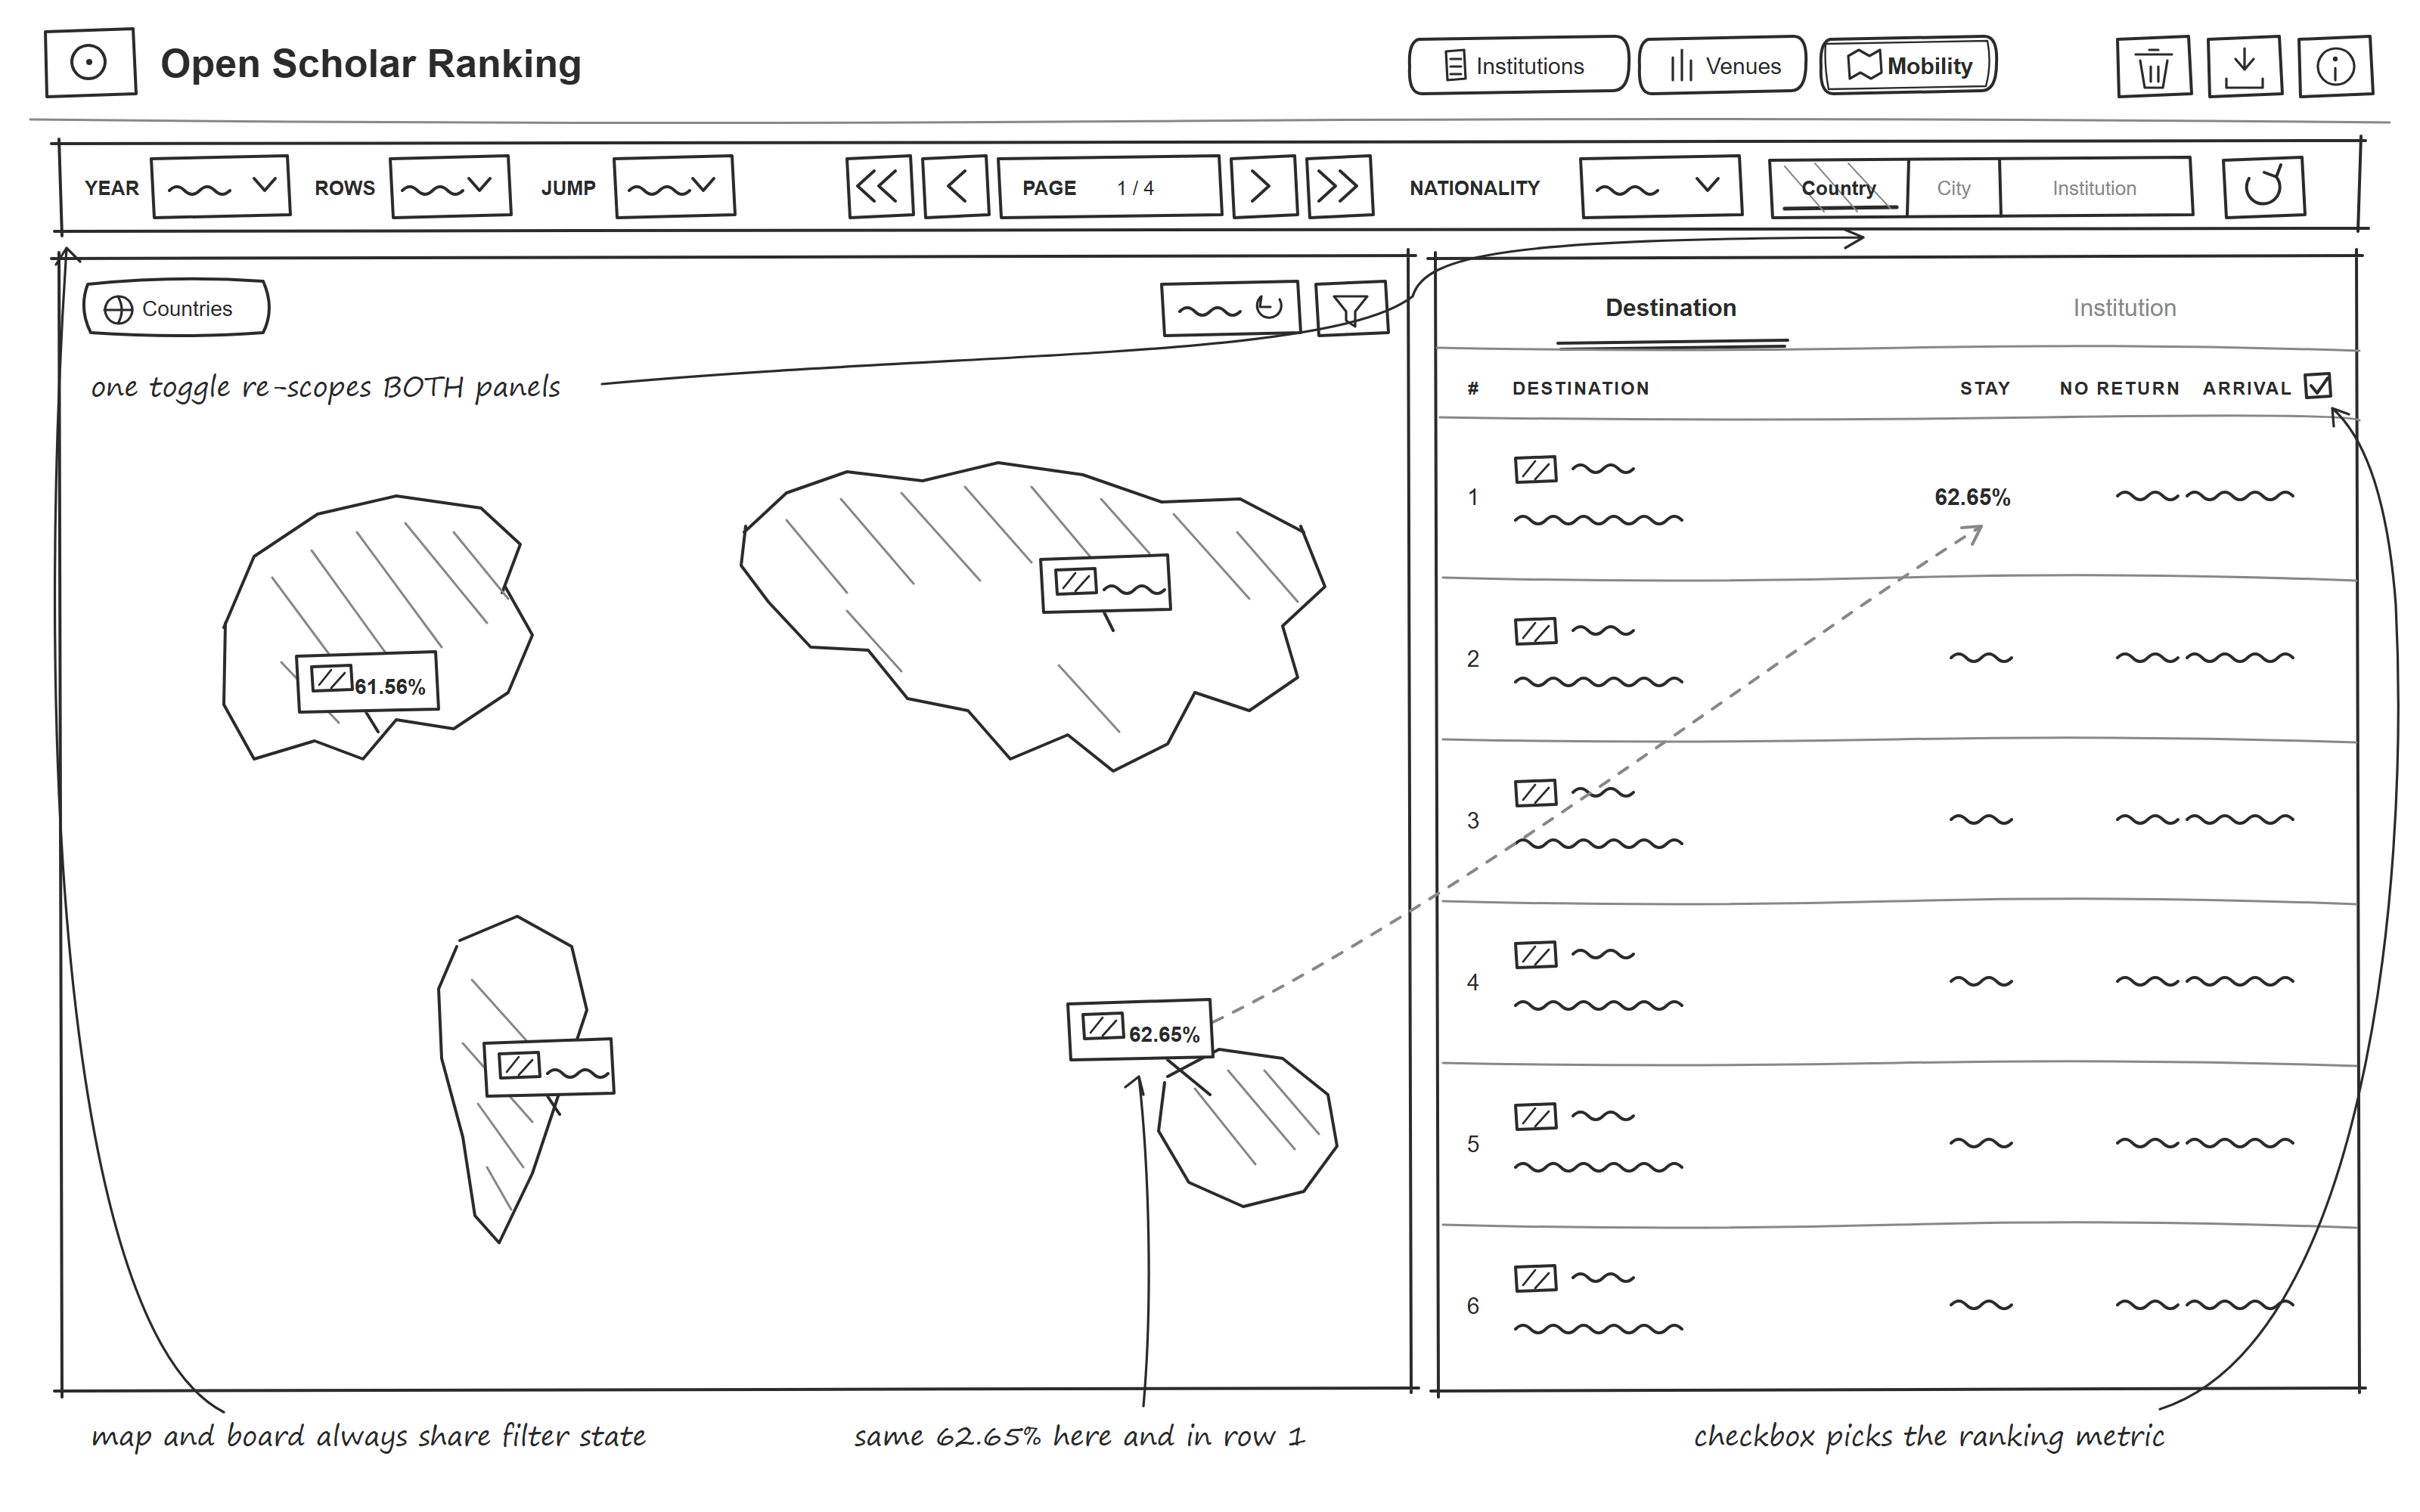
\includegraphics[width=0.68\linewidth]{figures/fig-w1.png}
\caption{W1, the mobility view. Map and destination board share one filter state, and a header checkbox picks the ranking metric.}
\label{fig:w1}
\end{figure}

\subsection{Evaluation}

\paragraph{Wireframe legibility check.} Each study session (Section~\ref{sec:iteration2}) opens with five minutes on the wireframes before the participant sees any live screen. They see W1 and W5 cold, say what each screen is for, show where they would click to answer ``which country is easiest for Chinese nationals to stay in'', and gloss the numbers they see. A note sheet records misreadings and stuck points \cite{nielsen1993usability}. This is a legibility check rather than a full walkthrough, and it runs after implementation. It tests whether the design's commitments read to first-time users, and its findings feed the next iteration rather than the already-shipped build. With three participants the check found no layout misreadings. All three read W1's purpose and the board's meaning cold, and two predicted the exact interaction path unprompted. What the sketches did not carry was semantics and labels. P02 read Stay as movement-anywhere rather than country-level retention until probed, flagged the country-code callouts as illegible for lesser-known countries, and expected sortable columns. P03's first instinct was to click a map country as a filter, an affordance the shipped design only grants on drilled views.

\paragraph{The launch as a field evaluation.} The implemented desktop design went public on 11 June 2026 on rednote and Reddit, and the coded launch corpus of Section~\ref{sec:pact} doubles as its field evaluation. Zone-level analytics bound its reach. It logged 15{,}010 unique visitors and 387{,}300 requests in the thirty days spanning launch, against a pre-launch baseline near 200 visitors a day, with daily traffic peaks on 13 June and around the sixth re-upload of 21 June. The posts accumulated roughly 40{,}000 likes and 35{,}000 saves (dashboards in Drive \texttt{07 Development evidence}).

Read as evaluation results, five findings dominate. Mobile was unusable (7 comments). The map would not zoom, data failed to load, layouts broke, and first contact happened on phones inside the rednote app. Small-sample anomalies drew ridicule (14 plausibility comments). ``Antarctica supposedly still has 38\% [staying]'' became the most-liked data critique in the corpus (735 likes), with Iraq's near-100\% Stay close behind. Rates shown without their underlying mass invite mockery. Metric confusion persisted (14 comments) over population scope and No-return semantics, despite the methodology page. Geographic merging errors (5 comments), administrative fragments presented as cities and opaque names like ``Staad'', anchored the top comment in the geo-merging theme (459 likes). The default flow filter hid entities silently (6 comments). One user read a filtered-out university as missing data. Four of the five are textbook heuristic violations \cite{nielsen1990heuristic}: the silent default filter breaks visibility of system status, metric confusion is a mismatch between the system and the real world, ambiguous absence forces recall where recognition should suffice, and the buried methodology gloss fails help and documentation.

Five decisions set the iteration-2 agenda: rebuild for touch as the primary platform, promoting W5 from sketch to spec; put a metric gloss one tap from every value; show the Arrival mass beside every rate and flag small samples; make active filters visible and let search bypass them; and resolve geographic entities with per-country localisation. Iteration 2 delivered the touch rebuild and the clarity work. The point-of-use gloss, the small-sample flag, and localisation stayed on the backlog, which the second evaluation confirms as the top fixes still ahead.
